\chapter{結果}
本章では,分子動力学法を用い粒子の振る舞いをシミュレーションし視覚化するプログラムの実行結果を記述する.

\section{作成したプログラム}
図\ref{fig:MDprogram}は本研究で作成したVerlet法とLennard-Jonesポテンシャルを用いて粒子の振る舞いをシミュレーションし,視覚化を行うプログラムである.
Processingで作成しているが,JavaScriptへ変換する事によってWebブラウザ上で動作させる事が可能である.
左の枠内に複数の粒子モデルが描画され,それらが枠内を動き回る.また,粒子の色を速度によって青から赤に変化させてエネルギーの推移をわかりやすくし,マウスカーソルで粒子をクリックしドラッグする事によって好きな方向に力を加える事ができる.
右側には2本のスライダーがあり,粒子の数とVerlet法の時間刻みを調整できる.
キー入力により状態を変更することができ,Sキーで凝固状態,Fキーで粒子に加わる力を視覚化した状態,Rキーで粒子のリセットを行うことができる.

\newpage
\begin{figure}[htbp]
 \begin{center}
  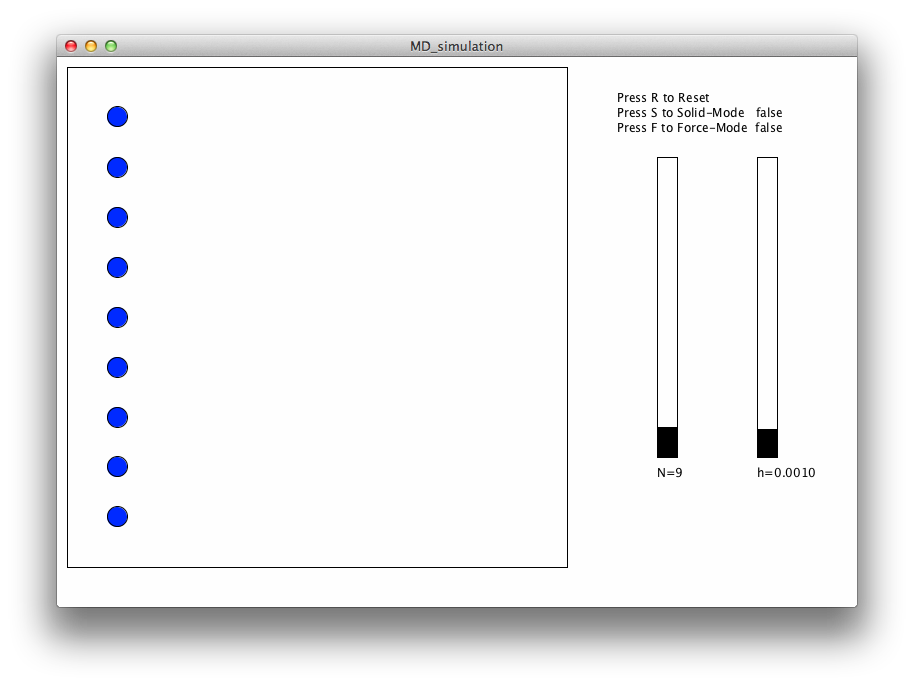
\includegraphics[width=150mm]{../implement/MDprogram.png}
 \end{center}
 \caption{分子動力学法視覚化プログラム.}
 \label{fig:MDprogram}
\end{figure}

\newpage

図\ref{fig:cluster}は粒子クラスタの移動を表しており,それぞれの粒子のクラスタとしての振る舞いを視認することができる.
スライダーで粒子の数を変更しマウスで力を加えることによって,このようなクラスタを好きなようにシミュレーションできる.
\begin{figure}[htbp]
 \begin{center}
  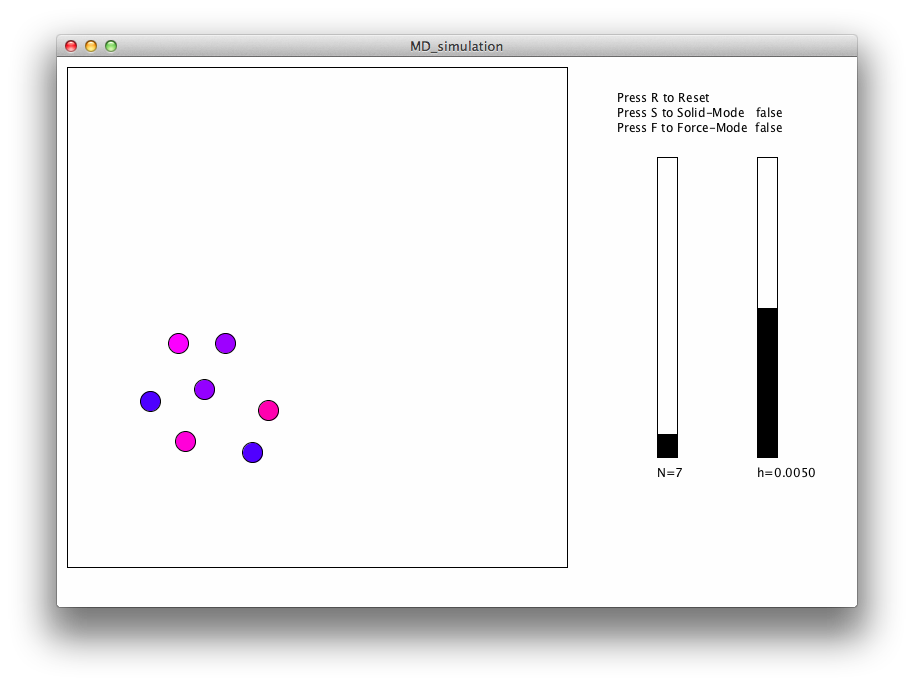
\includegraphics[width=150mm]{../result/cluster_picture.png}
 \end{center}
 \caption{クラスタの移動.}
 \label{fig:cluster}
\end{figure}


\newpage

図\ref{fig:solid}は凝固状態にしてしばらく実行し続けた結果であり,粒子が下の方に集まっていることが確認できる.これは粒子に下向きの力を継続的に加えて擬似的に凝固の現象を表現している.
これにより,粒子が自由に動き回る液体や気体の状態から,個体に移り変わる凝固現象の様子を確認できる.


\begin{figure}[htbp]
 \begin{center}
  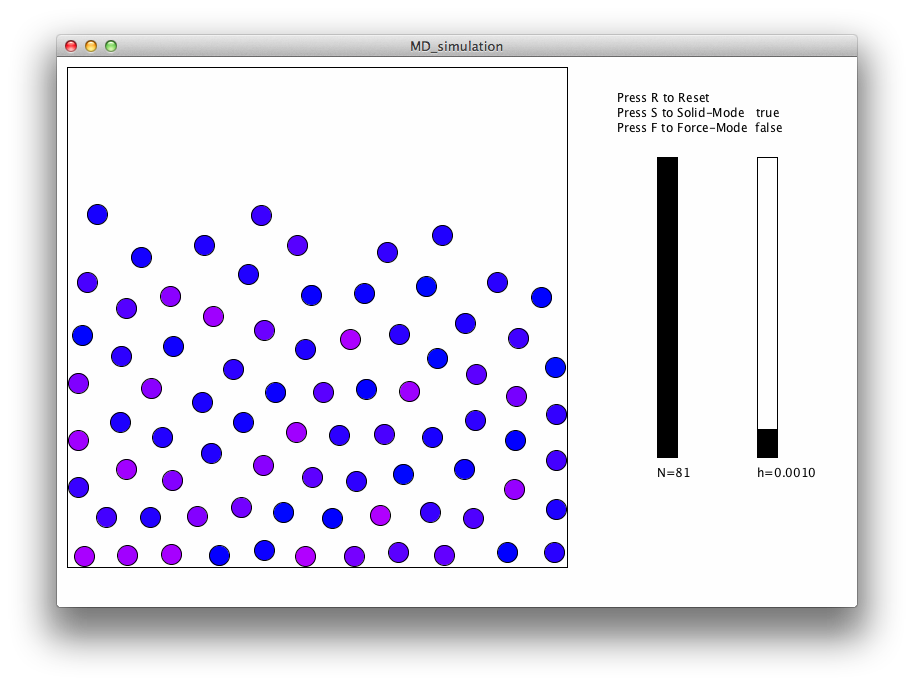
\includegraphics[width=150mm]{../implement/solid_mode.png}
 \end{center}
 \caption{凝固状態.}
 \label{fig:solid}
\end{figure}

\newpage

図\ref{fig:force}は粒子に加わる力を視覚化した状態であり,それぞれの粒子の中心から線が伸びている.
この線は長さが力の大きさ,向きが力の向きと対応しており力の加わり方をリアルタイムで把握することができる.
それぞれの粒子が力のパラメータを持っており,それらはシュミレーションの中で瞬時に変化していくため,値の確認は困難である.
しかし,この視覚化のおかげでそれぞれの粒子にかかる力を直感的に確認できる.

\begin{figure}[htbp]
 \begin{center}
  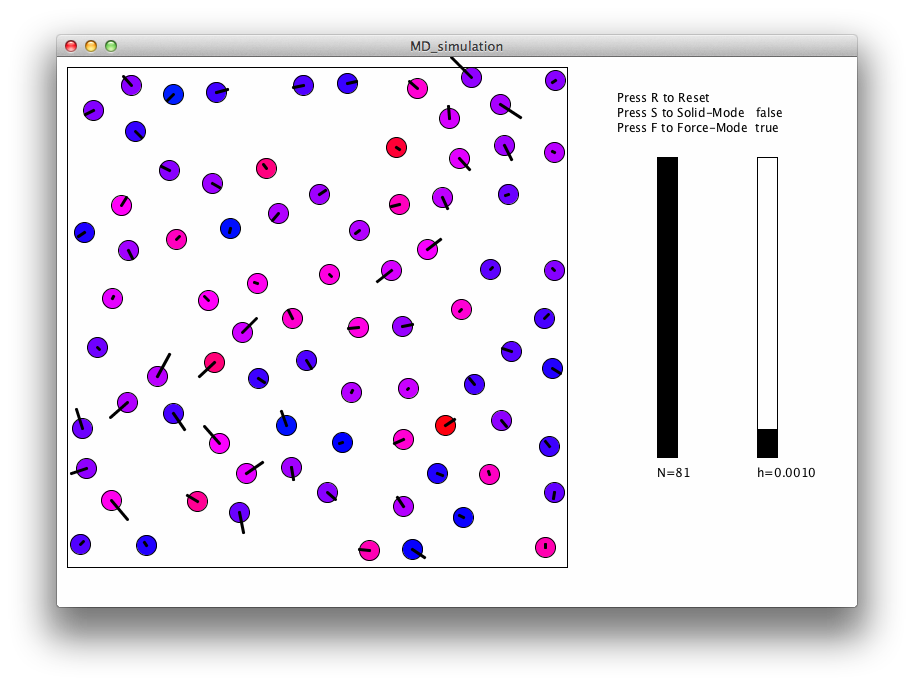
\includegraphics[width=150mm]{../implement/force_mode.png}
 \end{center}
 \caption{粒子に加わる力を視覚化した状態.}
 \label{fig:force}
\end{figure}
